\documentclass[14pt]{extarticle}
\usepackage[utf8]{inputenc}
\usepackage{ngerman}
\usepackage{array}
\usepackage{amsmath}
\usepackage{graphicx}
\title{Bericht Todesstern U5 - Transformationen}
\author{Charline Waldrich, Robert Ullmann, Julian Dobrot}
\date{15. Dezember 2015}

\begin{document}

\maketitle
\pagebreak
\tableofcontents

\section{Aufgabenstellung}
Implementierung von Samplings im Raytracer. Es soll zunächst ein Sampling Pattern erzeugt werden können, wobei die Punkte in einem regelmäßigen Raster angeordnet sind. Die Anzahl der Zeilen und Spalten können angegeben werden. Die Camera hat als weiteren Parameter ein Sampling Pattern. Die Methode rayFor gibt nicht länger einen einzelnen Strahl sondern eine Menge von Strahlen für einen Pixel zurück. Um die Farbe eines Pixels zu berechnen wird zunächst die Farbe für jeden Strahl ermittelt. Der Durchschnitt aller Werte genommen und dem Pixel zugewiesen. 
\subsection{Lösungsstrategien}
Übernehmen der Klassen Point2, Sampling Pattern aus dem UML Diagramm der Aufgabenstellung. Im Buch Raytrycing from ground up ist das Thema Sampling sehr ausführlich beschrieben. Die Grundlagen für die verschiedenen Samplingpattern und das grundlegende Verständniss des Samplings wurden auf Basis der im Buch thematisierten Algorithmen und Lösungen gebildet, da die Vorlesung zu dieser Thematik erst nach unserer ausarbeitung gehalten wurde.
\subsubsection{Implementierung}
Die ersten Schritte bei der Implementierung des Samplings in den Raytracer waren die Änderungen der Kamerakonstruktoren und das Programmieren der SamplingPattern Klasse an sich. Desweiteren musste der Rückgabetyp der rayFor Methode von Ray in ein Set von Rays geändert werden. Letztendlch musste noch  die ColorFor Methode die die Farbe für die einzelnen Pixel berechnet angepasst werden. Aus allen sich im Rayset befindenden Rays wird jetzt der Durchschnittswert berechnet, der den genaueren Farbwert des Pixels bestimmt.
\subsection{Probleme und besondere Ereignisse}
Auch wenn die Theorie die hinter dem Samplingprinzip steckt an sich recht trivial ist und auch die Algorithmen zu den eigentlichen Samplingtechniken in der Literatur sehr gut beschrieben sind, war die Sampling Implementierung sehr Zeitaufwendig. Da die Zusammenhänge zwischen den einzelnen Programmteilen im Raytracer zum Teil sehr komplex sind und erst nach eigener Programmierung verständlich werden. 
\subsection{Tests}
Die Abbildung zeigt normal gerenderte Scene.\\\\
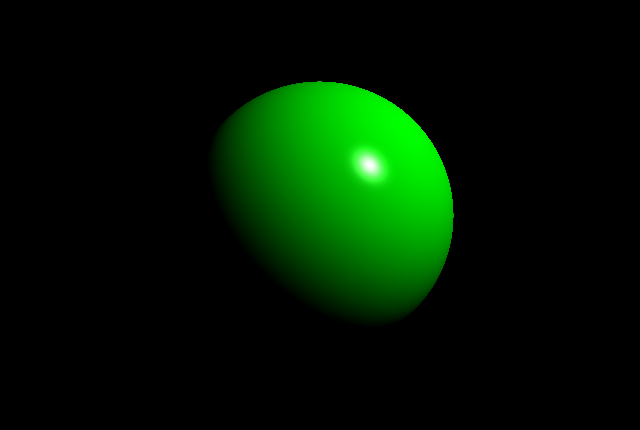
\includegraphics[width=15cm,height=10cm]{images/sample1.png}\\\\\\\\\\
Die Abbildung zeigt die Scene mit  regular Sampling 4x4.\\\\
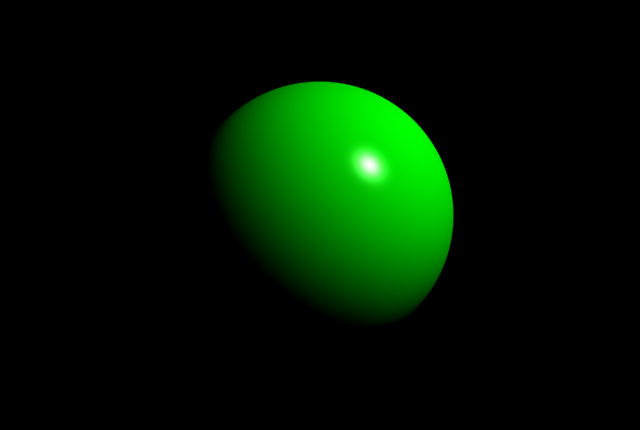
\includegraphics[width=15cm,height=10cm]{images/sample4x4.png}\\

\section{Zeitbedarf}
\begin{center}
\begin{tabular}{cr}

Implementiereung 	\	&180 min	\\
Programmierung \	&500 min	\\

Bericht  \		&40 min	 \\
	\hline
	&720 min
\end{tabular}
\end{center}

\section{Quellen}

\end{document}
